\chapter{Lasery półprzewodnikowe}
\section{Teoria}
\subsection{Teoria pasmowa}
Działanie laserów półprzewodnikowych opiera się na prawach, które opisuje teoria pasmowa.
Podstawowe przewidywanie teorii pasmowej mówi, że ciało stałe składa się z szeregu pasm rozdzielonych od siebie
przerwami energetycznymi o skończonych szerokościach. Najważniejszą przerwą, mającą wpływ na właściwości elektryczne ciała jest
przerwa pomiędzy pasmem walencyjnym i pasmem przewodnictwa $E_g$. Ze względu na szerokość przerwy
wyróżniamy~\cite{laser_book}:
\begin{itemize}
\item izolatory: $E_g > 3 \text{\,eV}$
\item półprzewodniki: $E_g = 0.1 \text{\,eV do } 2.5\text{\,eV} $
\item przewodniki: $E_g<0.1\text{\,eV}$
\end{itemize}

Przybliżoną wartość przerwy energetycznej w zależności od temperatury możemy przedstawić w postaci~\cite{laser_book}:
\begin{equation}
E_g(T) \approx E_{g0} - \frac{\alpha T^2}{\beta + T}
\end{equation}
gdzie: $E_{g0}$ --- wartość przerwy energetycznej w temperaturze $T=0$\,K,
Współczynniki $\alpha$ oraz $\beta$ są dodatnymi stałymi zależnymi od rodzaju materiału.
Dla $GaAs$ ~\cite{laser_book}: $\alpha = 4.5 \cdot 10^{-4}$\,eV, $\beta = 204$\,K.
Więc im wyższa temperatura tym wartość przerwy mniejsza.
\subsection{Lasery półprzewodnikowe}
Lasery półprzewodnikowe są ważną oraz dynamicznie rozwijająca się gałęzią optoelektroniki. Cały czas są one udoskonalane,
dzięki czemu obejmują coraz szerszy zakres częstości widma oraz potrafią generować promieniowanie o dużych mocach.
Zaletami laserów półprzewodnikowych są:
\begin{itemize}
\item małe wymiary,
\item łatwość modulacji emitowanego promieniowania,
\item niezawodność pracy,
\item proste zasilanie,
\item wymagane niskie napięcie zasilania,
\item stosunkowa niska cena w porównaniu do innych laserów.
\end{itemize}
W laserach półprzewodnikowych ośrodkiem aktywnym jest półprzewodnik.
Obszar czynny zazwyczaj ograniczony jest do wąskiego paska oraz położony jest w płaszczyźnie złącza p-i-n.
Pompowanie uzyskiwane jest przez wstrzykiwanie nośników ładunku do obszaru złącza, które spolaryzowane jest w kierunku przewodzenia.
Aby zaszła akcja laserowa, prąd zasilający musi przekroczyć pewną wartość progową zwaną prądem progowym $I_{\mathrm{th}}$, który w dalszej części jest
opisywany bardziej szczegółowo.
Podstawowym zjawiskiem fizycznym, na którym swe działanie opierają lasery półprzewodnikowe, jest przejście promieniste,
czyli proces rekombinacji elektronu i dziury, w wyniku którego następuje emisja promieniowania. Gdy prąd osiągnie wystarczająco
dużą wartość, dochodzi do inwersji obsadzeń.
Zajście inwersji obsadzeń pozwala wywołać akcję laserową. Wśród laserów półprzewodnikowych wyróżniamy:
lasery VCSEL oraz lasery o emisji krawędziowej.
\subsection{Laser VCSEL}
Laser VCSEL (ang. \textit{Vertical Cavity Surface Emitting Laser}) jest to laser z emisją powierzchniową o pionowej wnęce rezonansowej.
W laserach VCSEL promieniowanie rozchodzi się w kierunku prostopadłym do krawędzi obszaru czynnego oraz wzmacniane jest jedynie
wewnątrz tego obszaru \cite{publikcja_nakwaski}. Lasery tego typu zazwyczaj zbudowane są w kształcie pierścieni
lub walców o średnicach rzędu $\mathrm{\mu}$m.  Lasery VCSEL,   pracując   w   sposób   naturalny   na   pojedynczym   modzie  podłużnym,  charakteryzują się
znacznie lepszymi parametrami emitowanej wiązki promieniowania  niż
klasyczne  lasery krawędziowe \cite{publikcja_magda}. Emitowana wiązka ma małą rozbieżność kątową.
\begin{figure}[H]
\center
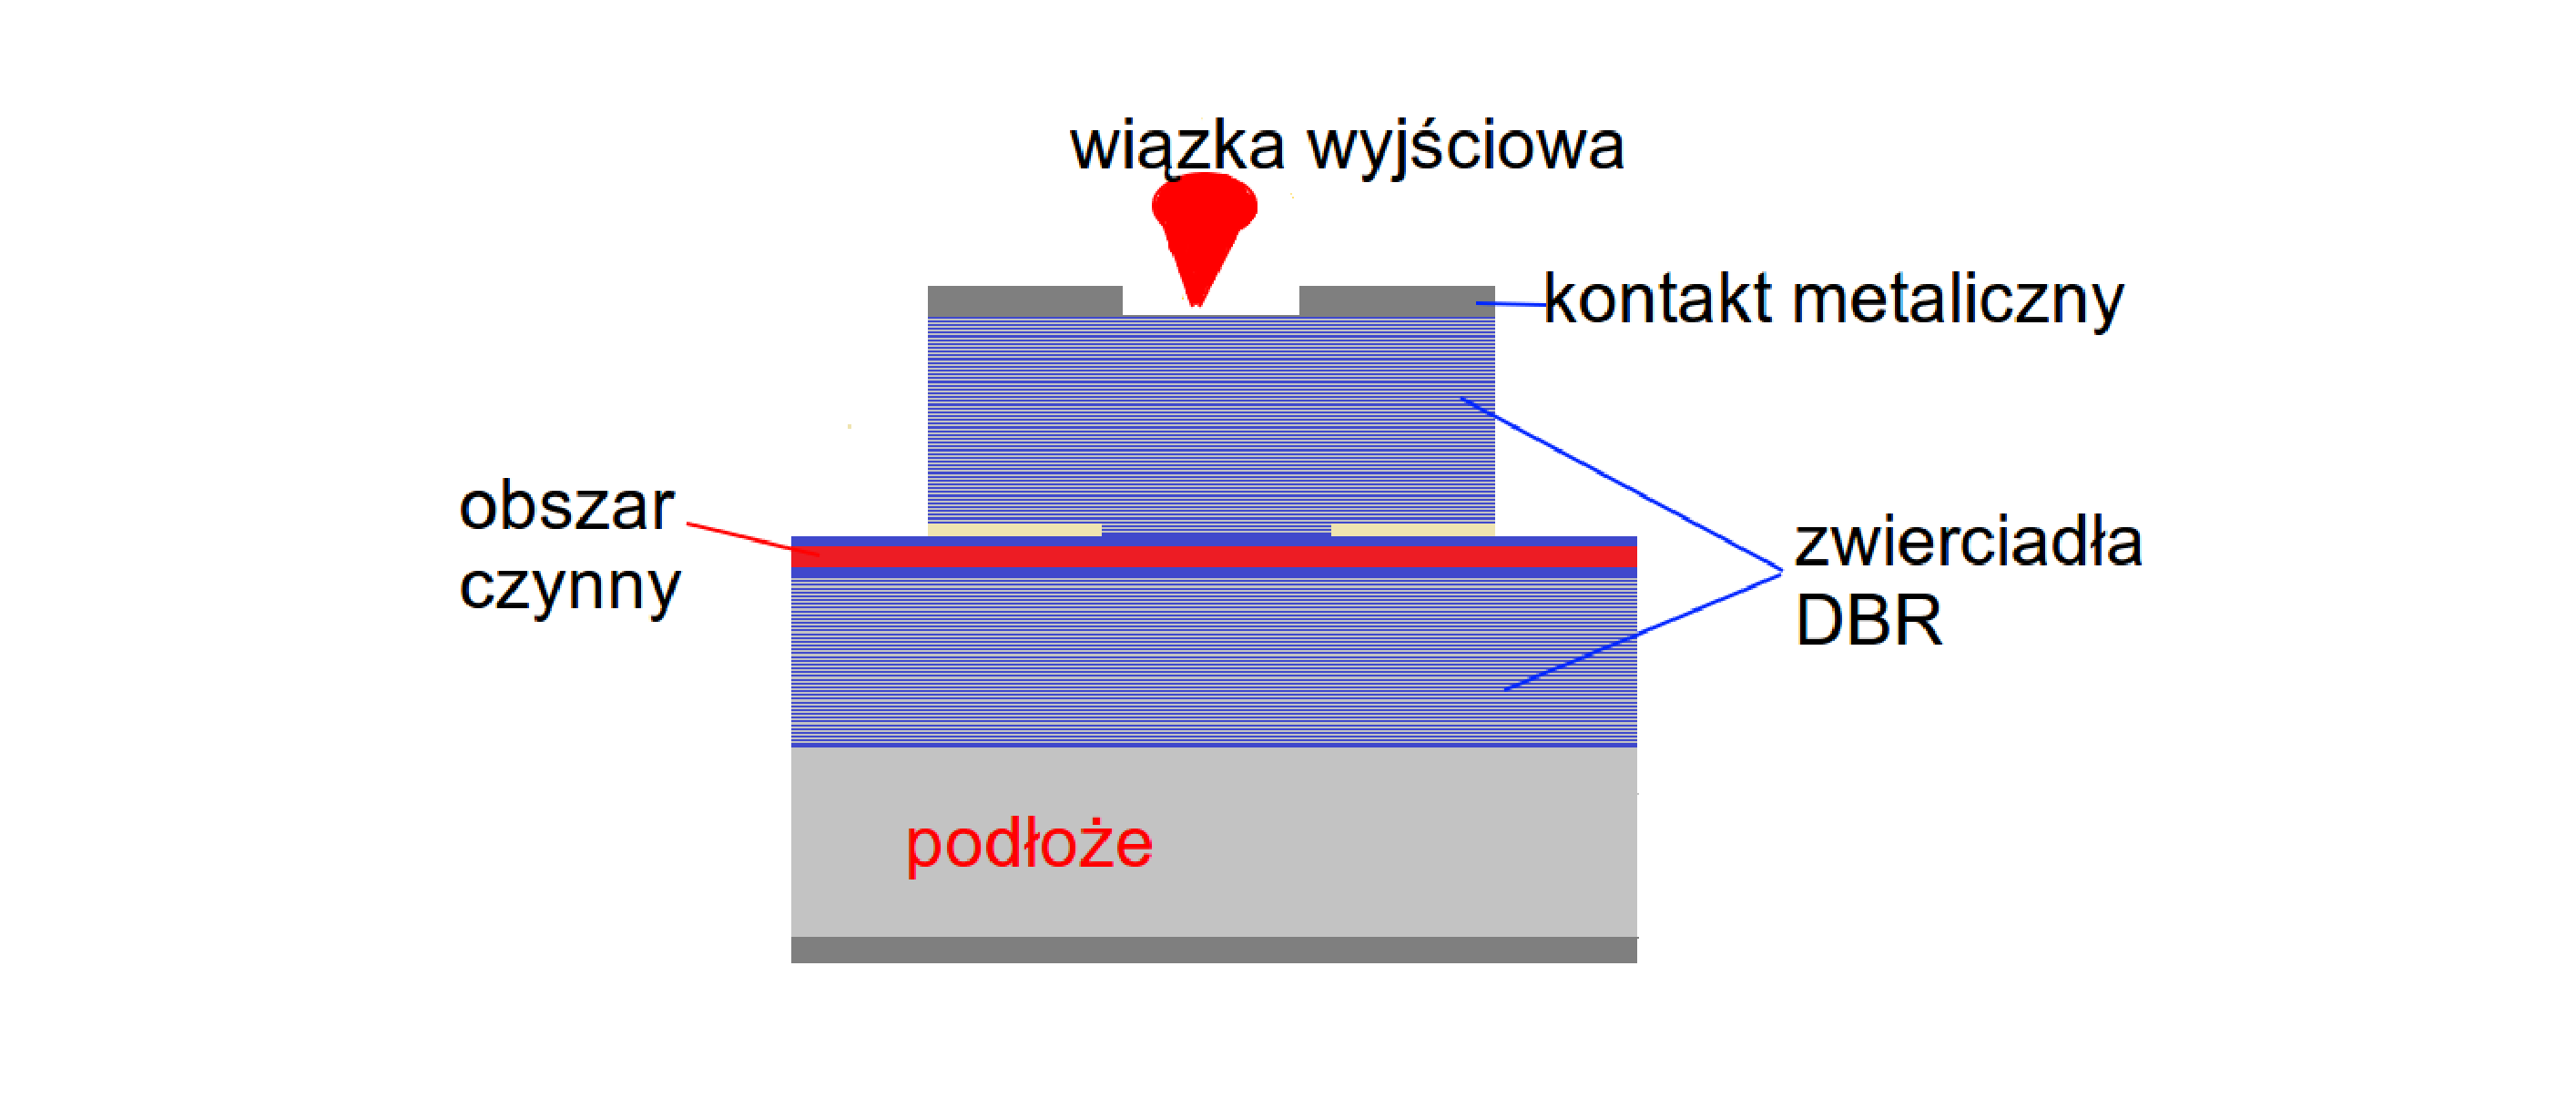
\includegraphics[scale=0.25]{vcsel2.eps}
\caption{Schemat budowy --- laser VCSEL.}
\label{fig:teoria_rys_3}
\end{figure}
Zaletami laserów VCSEL~\cite{publikcja_nakwaski} są:
\begin{itemize}
\item mała rozbieżność wiązki promieniowania,
\item naturalna praca na pojedynczym modzie podłużnym,
\item możliwość łączenia laserów w dwuwymiarowe matryce laserowe,
\end{itemize}
Wadami laserów VSCEL~\cite{publikcja_nakwaski} są:
\begin{itemize}
\item niska moc promieniowania wyjściowego (rzędu kilku \,mW),
\item Stosunkowa wysoka wartość oporności elektrycznej i cieplnej,
\item wzbudzanie się modów poprzecznych.
\end{itemize}
Zastosowanie laserów VCSEL:
\begin{itemize}
\item transmisja danych drogą optyczną,
\item spektroskopia absorpcyjna,
\item myszki komputerowe.
\end{itemize}
\subsection{Laser o emisji krawędziowej}
Laser krawędziowy jest to laser z wnęką w płaszczyźnie warstwy aktywnej. W tego typach laserach promieniowanie wędruje w rezonatorze między
jego zwierciadłami, jednocześnie cały czas znajdując się wewnątrz ośrodka czynnego. Odległości między modami jest mała.
Trudne jest otrzymania lasera krawędziowego pracującego na jednym modzie.
Rezonator jest zazwyczaj w kształcie prostopadłościanu o wymiarach niecałego milimetra, zazwyczaj wykonany także w materiale półprzewodnikowym\cite{publikcja_nakwaski}.
Sprężenie optyczne uzyskiwane jest przez zastosowanie pary zwierciadeł prostopadłych do płaszczyzny obszary czynnego lub
za pomocą pofałdowanej specjalnie powierzchni, która jest równoległa do tego obszaru (DFB --- Distributed Feed Back).
\begin{figure}[H]
\center
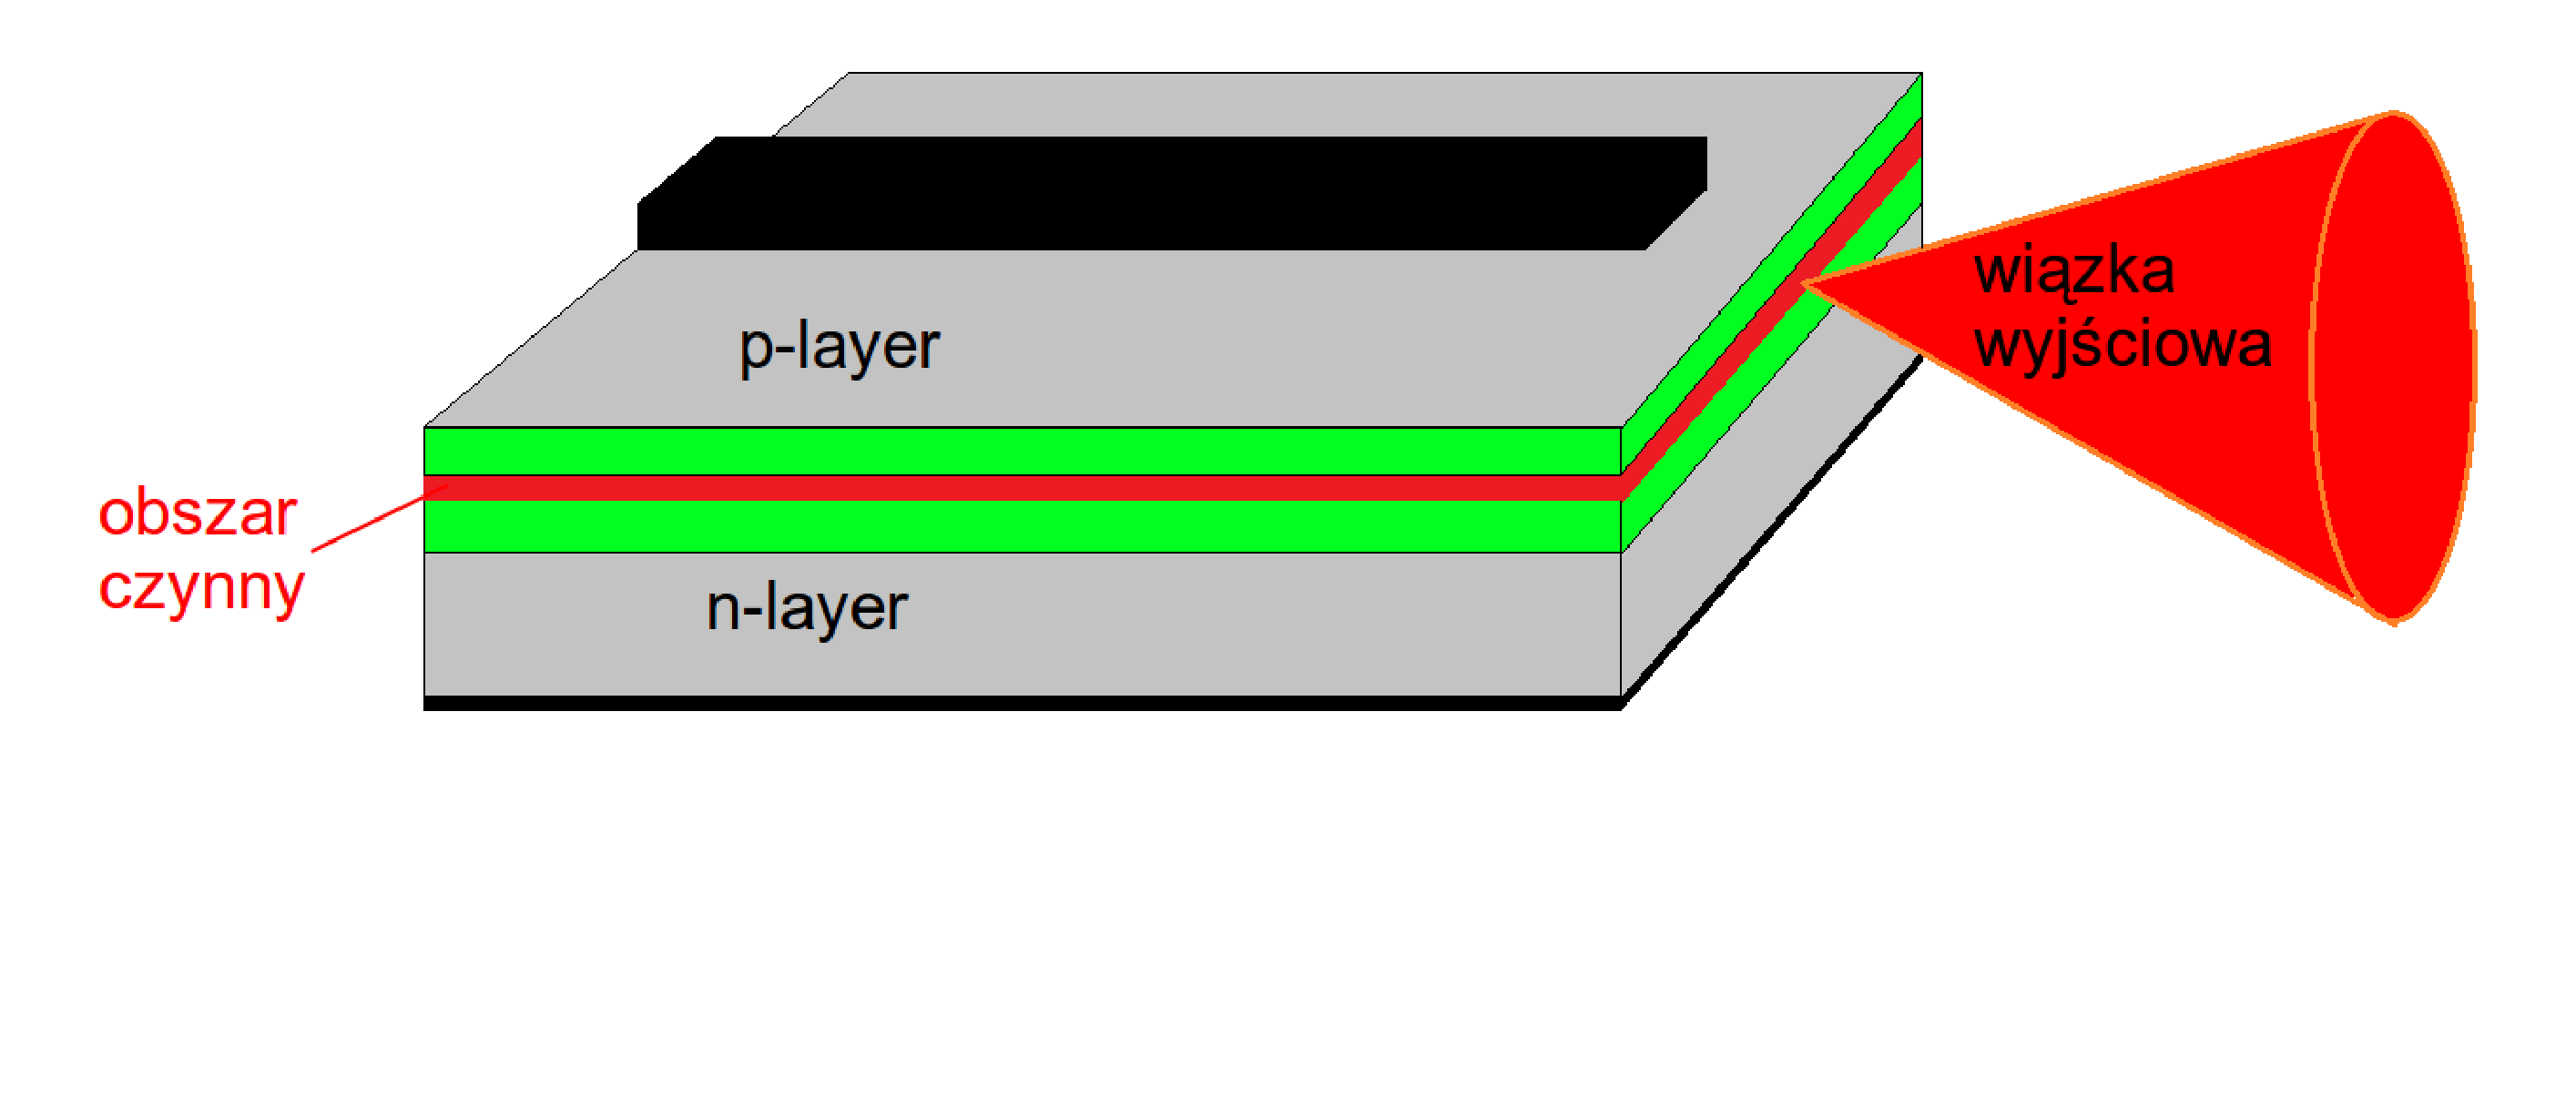
\includegraphics[scale=0.25]{kraw2.eps}
\caption{Schemat budowy --- laser krawędziowy.}
\label{fig:teoria_rys_3}
\end{figure}
Zaletami laserów krawędziowych są:
\begin{itemize}
\item stosunkowa wysoka moc wiązki wyjściowej \cite{publikcja_nakwaski} (do kilkadziesiąt mW),
\item stosunkowa wysoka sprawność,
\item możliwe łączenie laserów w jednowymiarowe matryce laserowe.
\end{itemize}
Wadami laserów krawędziowych są~\cite{publikcja_nakwaski}:
\begin{itemize}
\item wzbudzanie się wielu modów podłużnych,
\item rozbieżna wiązka promieniowania, która wykazuje astygmatyzm, zjawisko w którym promienie wiązki lasera padające w dwóch prostopadłych
płaszczyznach zostają zogniskowane w różnych punktach.
\end{itemize}
Zastosowanie laserów krawędziowych:
\begin{itemize}
\item w optyce światłowodowej do szybkiego przesyłania dużych ilości danych,
\item odczytywanie i zapisywanie płyt DVD.
\end{itemize}
\newpage
\subsection{Prąd progowy}
Charakterystyka wyjściowa lasera przedstawia zależność napięcia na laserze oraz mocy wyjściowej w funkcji prądu zasilającego.
Ważnym parametrem laserów półprzewodnikowych jest prąd progowy (ang. \textit{threshold
current}) który określa wartość prądu, przy którym zaczyna zachodzić akcja laserowa, czyli
rośnie gwałtownie natężenie promieniowania i maleje szerokość linii emisyjnej. W celu wyznaczenia prądu progowego należy
sporządzić wykres zależności mocy wyjściowej lasera od prądu zasilającego. Następnie dla kawałka liniowego zależności prądu
od mocy wyjściowej, gdzie moc wyjściowa gwałtownie rośnie, metodą najmniejszych kwadratów przy użyciu prostej (\ref{eq:fit_i_th}) należy
znaleźć parametry prostej $a$ i $b$.
Dla wyznaczonej prostej należy znaleźć miejsce zerowe, które będzie wyznaczoną wartością prądu progowego $I_{\mathrm{th}}$(\ref{eg:i_th}).
\begin{equation}
\label{eq:fit_i_th}
P_{\mathrm{wy}} = a \cdot I + b
\end{equation}
\begin{equation}
\label{eg:i_th}
I_{\mathrm{th}} = -\frac{b}{a}
\end{equation}
\begin{equation}
\Delta I_{\mathrm{th}} = \left\lvert \frac{\partial I_{\mathrm{th}}}{\partial a} \right\rvert \cdot \Delta a + \left\lvert \frac{\partial I_{\mathrm{th}}}{\partial b} \right\rvert \cdot \Delta b
\end{equation}
\begin{equation}
\Delta I_{\mathrm{th}} = \left\lvert -\frac{b}{a^2} \right\rvert \cdot \Delta a + \left\lvert -\frac{1}{a} \right\rvert \cdot \Delta b
\end{equation}
Dla laserów krawędziowych prąd progowy rośnie wraz z temperaturą.
Zależności prądu progowego $I_{th}$ od temperatury $T$ wyrażamy w postaci równania:
\begin{equation}
\label{eq:i_th}
I_{\mathrm{th}} = I_0 \exp \left( \frac{T}{T_0} \right)
\end{equation}
Przez zlogarytmowanie wartości prądu oraz podstawienie otrzymujemy:
\begin{equation}
\ln(I_{\mathrm{th}}) = \frac{T}{T_0} + \ln(I_0)
\end{equation}
Wartości parametrów $I_0$ oraz $T_0$ możemy wyznaczyć na podstawie charakterystyk
emisyjnych lasera w różnych temperaturach $T$. Parametr
$T_{0}$ wyrażomy w kelwinach jest to tzw. temperatura charakterystyczna~\cite{opto_book}.

Mając wartości prądu progowego w danej temperaturze można do nich dopasować funkcje liniową o parametrach $k$ i $w$ w postaci:
\begin{equation}
y = k \cdot T + w
\end{equation}
gdzie:
\begin{equation}
y = \ln(I_{\mathrm{th}})
\end{equation}
\begin{equation}
k = \frac{1}{T_0}
\end{equation}
\begin{equation}
w = \ln(I_0)
\end{equation}
Na tej podstawie możemy znaleźć poszukiwane parametry $I_0$ oraz $T_0$:
\begin{equation}
I_0 = \mathrm{e}^w
\end{equation}
\begin{equation}
T_0 = \frac{1}{k}
\end{equation}
Korzystając z metody różniczki zupełnej można obliczyć wartości błędów wyznaczonych wartości:
\begin{equation}
\Delta I_0 = \left\lvert \frac{\partial I_{0}}{\partial w} \right\rvert \cdot \Delta w = | \mathrm{e}^w | \cdot \Delta w
\end{equation}
\begin{equation}
\Delta T_0 = \left\lvert \frac{\partial T_{0}}{\partial k} \right\rvert \cdot \Delta k = \left\lvert -\frac{1}{k^2} \right\rvert \cdot \Delta k
\end{equation}
Dla laserów VCSEL nie można zastosować zależności (\ref{eq:fit_i_th}).
\subsection{Sprawność}
Innym ważnym parametrem, którym możemy scharakteryzować lasery półprzewodnikowe, jest ich sprawność. Mnie interesować będą
następujące rodzaje sprawności:
\begin{itemize}
\item Sprawność różniczkowa (ang. \textit{slope efficiency}) --- jest zdefiniowana jako nachylenie krzywej uzyskanej przez wykreślenie zależności
mocy wyjściowej $P_{wy}$ z lasera w funkcji natężenie prądu $I$ lub mocy dostarczonej $P_{we}$.
Moc dostarczoną definiujemy jako:
\begin{equation}
P_{we} = U \cdot I
\end{equation}
gdzie: $U$ --- napięcie na laserze.
Sprawność różniczkowa jest pochodną mocy wyjściowej po prądzie $\frac{dP_{wy}}{dI}$ lub pochodną mocy wyjściowej po mocy wejściowej $\frac{dP_{wy}}{dP_{we}}$
\item Sprawność całkowita (ang. \textit{wall-plug-efficiency}) --- jest zdefiniowana jako stosunek mocy wyjściowej do całkowitej mocy wejściowej lasera.
\begin{equation}
\eta = \frac{P_{wy}}{P_{we}}
\end{equation}
Wyznacza się ją przez podzielenie mocy wyjściowej $P_{\mathrm{wy}}$, czyli zmierzonej na mierniku mocy przez moc wejściową $P_{\mathrm{we}}$
\end{itemize}